%file included in thesis.tex


\chapter{Data Representation and Interpretation}
\label{chap5}
Choosing how to represent the world is an important design parameter of the system. The
robot is have limited space and computational abilities, therefor the representation
should not be too spacious in the control systems memory. If one allows reasoning in the
system, the space of the representation becomes less, but the complexity of the reasoning
and sensor interpretation increase. With increased reasoning, the possibility for the
control system to take the wrong decision becomes substantial, and the integrity of the
map building compromised. Summarized, the more abstract representation, the more reasoning
of the control system are needed, but the representation takes less space in the control
systems memory. 

\section{World Representation}
The world representation should have a number of qualities. First it must represent the
world in a satisfactory way. It should be easy to update and take up little memory on the
implementation platform. Third it should be easy to understand for a human operator
without too much post-processing. 

The possibility of global positioning must be met. The robot must be able to match its
created map to a \`a priori map.

The problem when a robot has to reason, is that it might
take the wrong decisions, and the risk of erroneous map making are high. 

\subsection{Nodes}
The representation in this project is a kind of topological map. It is abstract in the way
that the world are classified into given nodes. Known features of the world are recognized
and represented as nodes in a graph. 

This means that the world need to be classified into predefined nodes before the mission
is started. In this project the nodes are junctions, or bends that are easily recognized
because of their fundamental difference to the straight pipe segments. 

The nodes should have a number of attributes describing how the node is different from the
other nodes. These attributes are:
\begin{itemize}
    \item Node type
    \item Number
    \item Time stamp when discovered
    \item Previous Node
    \item Distance since last node
    \item Orientation
    \item Number of edges and the angles of those
    \item List of anomalies
\end{itemize}

Most of this attributes are self-explaining, but the last attribute, \emph{list of
anomalies} deserves a closer explanation. 
Anomalies are those things that the robot should look after, and record. An anomaly are
everything that is not expected. In a pipe environment the surroundings are assumed to be
in some way, because they are designed that way. Everything that is not as expected should
be recorded for later inspections. 

This list will contain every anomaly from the previous node to the next one, where the
list is stored. The list will contain a time stamp of when it was discovered, distance
traveled from the previous node, and a remark why it was detected as an anomaly. Since
this involves a lot of reasoning by the control system, theres a chance that actual
pipeline junctions might be marked as anomalies instead of being recognized as nodes.

Because the anomalies are detected before the node that will contain the list are
detected, the list is temporary stored in the robots memory until the next node are
detected. 
\begin{figure}[htbp]
    \centering
    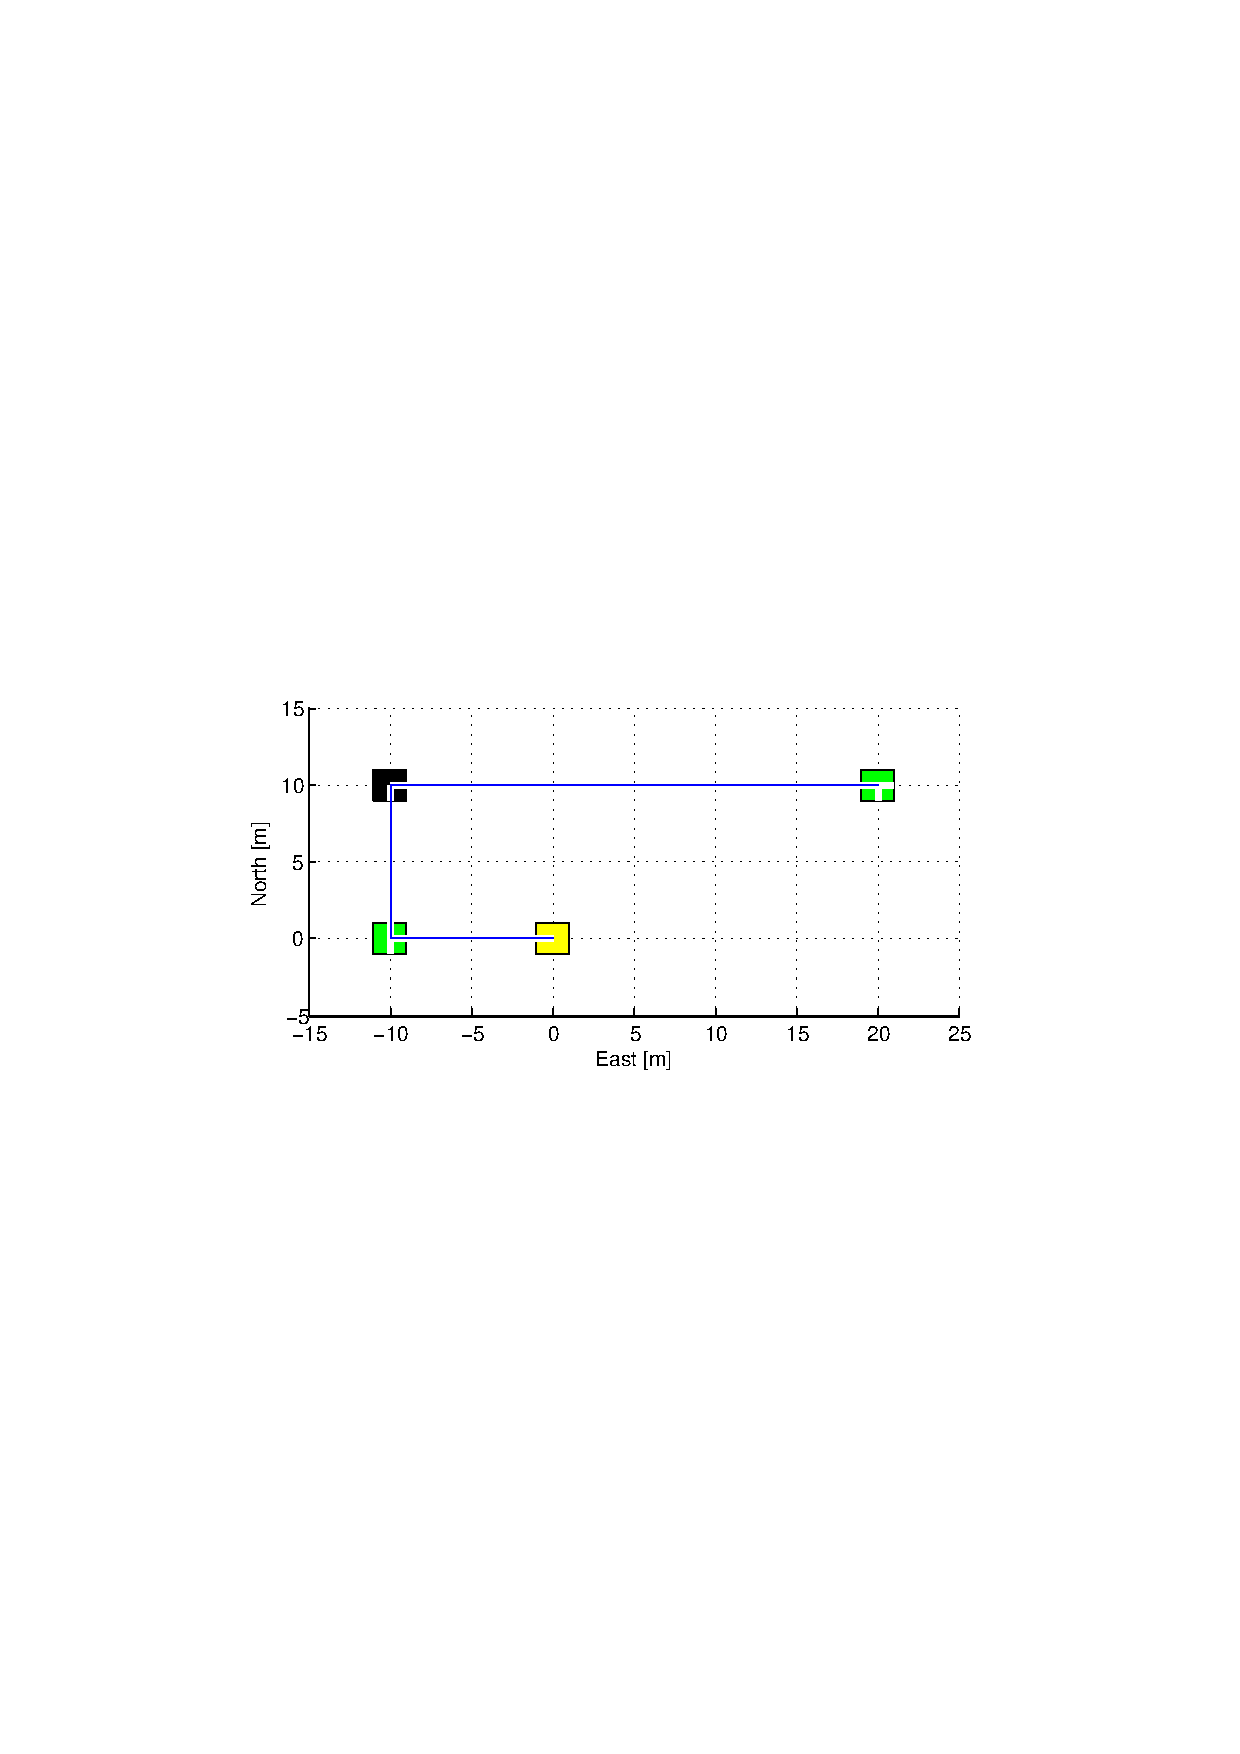
\includegraphics[width=0.8\textwidth]{pics/worldrepresentation}
    \caption{An example of the world representation}
    \label{chap5:fig-worldrepresentation}
\end{figure}


\section{Map-building From the Sensor Data}


\subsection{Cylinder Fit from 3D Sensor Data}
The three dimensional point cloud which is output form the Time-of-Flight camera are
filtered before it is fed to the surface fit algorithm. Firstly the intensity images, is
used for filtering out pixels with too high or too low intensity values. The high
intensity values indicate that the pixel is too close to measure, or that the surface is
too reflective, either way this will give bad range data. The pixels which have too low
intensity values are either too far away, or might indicate that a multi-path reflections
and are filtered away. 

After doing this a number of successive captures are averaged to provide less noisy image.
Then the coordinates are sorted on the z-coordinate and divided into $n$ equally spaced
subsets. This means that there will be $n$ cylinders fitted to the captured point cloud.
This is too ease the amount of memory used to process the whole point cloud, which as
shown later was to big much for matlab to handle. 

The surface fit algorithm is a Nonlinear Least-Squares Guass-Newton algorithm. It parameterize the
cylinder as described in Section \ref{chap2:sec-surface-fit-alg}. The input to this
algorithm is start coordinates of the cylinder axis, $x_0$, the axis direction $a_0$, and
the initial radius, $r_0$.

\begin{algorithm}[htbp]
    \caption{Cylinder Fit Algorithm}
    \label{chap5:alg-cylinderfit}
    \begin{algorithmic}
        \REQUIRE (X, Y, Z) $\leftarrow$ point cloud and IntensityImage
        \STATE Filter pixels with intensity values below $LowIntensity$ and $HighIntensity$
        \STATE Average point cloud over $x$ samples
        \STATE Remove all trivial points
        \STATE Sort on Z-coordinate
        \STATE Divide point cloud into $n$ equally spaced $SubSets$
        \FOR{every $SubSets$}
            \STATE Get initial values for Surface Fit algorithm
            \STATE  $r, a, x_0, d$ $\leftarrow$ run surface fit algorithm on $SubSets$
        \ENDFOR
        \FOR{every $r$}
            \IF {$r > m \times PipeRadius$}
                \STATE Mark $r$ as erroneous
            \ENDIF
        \ENDFOR
    \end{algorithmic}
\end{algorithm}

Here there are a couple of problems. First, the points not belonging to the geographical
primitive, i.e. the cylinder will draw the cylinder fit off-axis, and cause the cylinder
fit to fail, as the Least-Squares approach assumes that all the points in the supplied set
belongs to the cylinder. The algorithm are guaranteed to converge if the term $J_k^T J_k$
dominates the approximation to the Hessian which is used in the Gauss-Newton algorithm
described in Section \ref{chap2:subsec-gauss-newton}. \cite{optreg}

The user parameters in this algorithm are the \emph{subset threshold} which decides the interval
of the subsets and also how many cylinders should be fitted to the given point cloud. The
other parameters are $m$ which tells for which values the predicted cylinder radii are
erroneous. 

The initial values which are required for the surface fit, is the assumed start position
of the cylinder which at the first \emph{SubSet} is at the origin with regard to the
ToF-camera sensor frame, and the initial axis which unless other is said is along the
z-axis, i.e. into the pipe seen from the camera.


\subsection{Line Fit in 2D Sensor Data}
Line fit algorithm is a least-squares line fit algorithm. For this to work properly, a
selection of points assumed belonging to the line need to be fed into the algorithm. To
select this points a histogram is formed for both x- and y-direction of the points. This
will detect points which lie in a horizontal- and vertical lines. This points are selected
and fed into the line fit algorithm. 

This approach is also prone to the problem with least squares, that all the points are
assumed to belong to the geographical primitive, and that the noise averages out when
enough samples are taken. But here the points are segmented on vertical and horizontal
lines. Lines that are neither horizontal or will causes problem for this algorithm. If the
histogram bins are too large, the direction of the fitted line will be diverted, and if it
is too small the algorithm will not detect the points as a belonging to a line. 
\begin{algorithm}[htbp]
    \caption{2D Line Fit algorithm}
    \label{chap5:alg-2dlinefit}
    \begin{algorithmic}
        \REQUIRE $(r, \theta)$ from Laser Range Finder
        \STATE average $r, \theta$ over $n$ samples
        \STATE convert $r, \theta \rightarrow$ $x, y$ 
        \STATE with regard to $y$ construct histogram with $hist_y$ intervals
        \FOR{each $Bin$ in $HitogramY$}
            \IF{Number of points in $Bin$ $>$ $NoPointsY$}
                \STATE Pass these points to the Least-Squares Line Fit Alg $\rightarrow$ $a_y$, $b_y$
            \ENDIF
        \ENDFOR
        \STATE with regard to $x$ construct histogram with $hist_x$ intervals
        \FOR{each $Bin$ in $HitogramX$}
            \IF{Number of points in $Bin$ $>$ $NoPointsX$}
                \STATE Pass these points to the Least-Squares Line Fit Alg $\rightarrow$ $a_x$, $b_x$
            \ENDIF
        \ENDFOR
    \end{algorithmic}
\end{algorithm}

Parameters needed to be set by the user is, the histogram bin sizes, $hits_x$ and
$hits_y$. The more points will fit into the bins, and the lines will be more prone to
other points that does not ``belong'' to the wall points. The other parameters are the
threshold parameters for how many points there need to be in a histogram bin to pass them
to the line fit, $NoPointsX$ and $NoPointsY$.

From these lines the radius and direction of the pipe can be found. The position of the
Laser Range finder is assumed known, particularly the height above the ground are needed
to calculate the radius of the pipe. The following relation is used.
\begin{align}
    r^2 &= P_2^2 + \left(\frac{d}{2} \right)^2 \\
    r &= P_1 + P_2  \quad \rightarrow \quad P_2 = r - P_1
\end{align}
       Where $r$ is the radius of the pipe, $P_1$ is the distance from the measurement plane to
the lowest point in the pipe, $P_2$ is the distance form the center of the pipe to the
measurement plane and $d$ is the distance between the matched line segments. Substituting
for $P_2$ and rearranging
\begin{equation}
    \begin{aligned}
        r^2& = (r - P_1)^2 + \left(\frac{d}{2}\right)^2 = r^2 - 2 r P_1 + P_1^2 +
        \left(\frac{d}{2}\right)^2 \\
        2 r P_1 &= P_1^2 + \left(\frac{d}{2}\right)^2 \\
        r &= \frac{P_1}{2} + \frac{d^2}{8 P_1}
    \end{aligned}
\end{equation}
This requires that two lines can be matched to be approximately parallel for the distance
$d$ to be calculated. Therefor the direction of all the lines are compared to all the
other lines and those parallel within some threshold, $ParallelThreshold$ are selected.


\section{Positioning in the World Representation}
How the control system positions itself in the environment is very important for the
control system. Because the system need to know where it is, and where it has been, to be
able to determine where it will go. 

Given the case that the \emph{SensorInterpreter} is capable of identifying and matching
the nodes correct, this can be used as landmark when determining global position. The
graph which have been created, can be matched with the \`a priori map, based on what kind
of nodes that have been passed, the taken path of the robot can be matched given that the
\`a priori map is accurate with regard to the location and order of the nodes. 

For example the robot passes first through a L-bend, then continues to a Y-Junction. It
continues to the left, where it hits a R-bend and into a T-Junction. This sequence of
nodes, can be matched to the given map, and a position can be estimated. If there are
ambiguities the correct position cannot be established before additional nodes are passed.
The pipe network need to be, using an analogue to the system identification terminology, 
\emph{persistently exciting}. Which means that the network consists of enough unique features and
sequences that the position can be determined uniquely. 

********REFERENCE TO MAKRO which uses this kind of positioning*********

